\documentclass[problem]{mcs}

\begin{pcomments}
  \pcomment{PS_koch_induction}
  \pcomment{DRAFT: FORMULAS ARE WRONG}
  \pcomment{elaboration of PS_koch_snowflake}
  \pcomment{ARM 4/8/14}
\end{pcomments}

\pkeywords{
  induction
  equilateral
}

%%%%%%%%%%%%%%%%%%%%%%%%%%%%%%%%%%%%%%%%%%%%%%%%%%%%%%%%%%%%%%%%%%%%%
% Problem starts here
%%%%%%%%%%%%%%%%%%%%%%%%%%%%%%%%%%%%%%%%%%%%%%%%%%%%%%%%%%%%%%%%%%%%%

\begin{problem}

Let's define a sequence of polygons $S_0, S_1$ recursively, starting
with $S_0$ equal to a unit square.  We construct $S_{n+1}$ by removing
the middle third of each edge of $S_n$ and replacing it with two line
segments of the same length, as illustrated in Figure~\ref{kochline}.
Let $a_n$ be the area of $S_n$.  So $a_0 =1$ and $a_1$ equals $a_0$
plus the area of four equilateral triangles with side 1/3.  Namely,
\[
a_1 = 1 + 4 \cdot \frac{\sqrt{3}}{2}\paren{\frac{1}{3}}^2.
\]

Prove by induction that
\begin{staffnotes}
NOT RIGHT:
\end{staffnotes}

\begin{equation}\label{an1s3}
      = 1+ \frac{\sqrt{3}}{4}   \paren{\frac{1 - (4/9)^n}{5}}
  a_n = 1 + \sqrt{3} \frac{1 - (4/9)^n}{20}.
\end{equation}

\begin{staffnotes}
\hint
\[
a_{n+1} = a_n + \frac{\sqrt{3}}{4}e_n\, (l_{n+1})^2
\]
\end{staffnotes}

\begin{figure}
  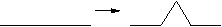
\includegraphics[width=2.5in]{koch}
  \caption{Constructing the Koch Snowflake.}
  \label{kochline}
\end{figure}

\begin{solution}
From the definition of $S_{n+1}$, we have
\begin{align}
l_{n+1} & = \frac{l_n}{3},\label{ln+13}\\
e_{n+1} & = 4e_n,\label{en+14}\\
a_{n+1} & = a_n + \frac{\sqrt{3}}{4}e_n (l_{n+1})^2.\label{an+1a}
\end{align}

So
\begin{equation}\label{ln/en}
l_{n+1} = 3^{-(n+1)},\qquad e_{n+1} = 4^{n+1},
\end{equation}
which could be verified a trivial induction.

We now use~\eqref{an+1a} to prove by induction on $n$
that~\eqref{an1s3} holds for all $n$, with~\eqref{an1s3} serving as
induction hypothesis.

\begin{proof}
\inductioncase{Base case}: ($n=0$) We start with the unit square, so
$a_0=1$.  The right hand side of~\eqref{an1s3} is $1+ \sqrt{3}
\paren{\frac{1 - 1}{5}} = 1$, as required.

\inductioncase{Induction step}: \TBA{CHECK THE ALGEBRA}

\end{proof}

By the way, we derived~\eqref{an1s3} using the formula for a geometric sum:
\begin{align*}
a_{n+1} & =  a_n +  \frac{\sqrt{3}}{4}4^n 9^{-(n+1)}\\
  & = 1 + \frac{\sqrt{3}}{4^2}\sum_{k=1}^{n+1} \paren{\frac{4}{9}}^k.
\end{align*}

\iffalse
  & = 1+ \frac{\sqrt{3}}{4^2} \paren{\frac{1 - (4/9)^{n+2}}{1-4/9} - 1}\\
  & = 1+ \frac{\sqrt{3}}{4^2} \paren{\frac{4 - 4(4/9)^{n+1}}{5}}\\
  & = 1+ \frac{\sqrt{3}}{4}   \paren{\frac{1 - (4/9)^{n+1}}{5}}
\fi


So as $n$ goes to infinity, the area $a_n$ approaches $1+ \sqrt{3}/5$
while the perimeter approaches a nowhere differentiable curve whose
length is $\lim_{n \to \infty} e_n l_n = \lim_{n \to \infty} (4/3)^n =
\infty$.

\end{solution}

\end{problem}

%%%%%%%%%%%%%%%%%%%%%%%%%%%%%%%%%%%%%%%%%%%%%%%%%%%%%%%%%%%%%%%%%%%%%
% Problem ends here
%%%%%%%%%%%%%%%%%%%%%%%%%%%%%%%%%%%%%%%%%%%%%%%%%%%%%%%%%%%%%%%%%%%%%

\endinput

